\RequirePackage[T1]{fontenc}
\documentclass[conference]{IEEEtran}
\IEEEoverridecommandlockouts

\usepackage{cite}
\usepackage{amsmath,amssymb,amsfonts}
\usepackage{algorithmic}
\usepackage{algorithm}
\usepackage{graphicx}
\usepackage{textcomp}
\usepackage[english]{babel}
\usepackage[dvipsnames]{xcolor}
\usepackage{booktabs}
\usepackage{tabularx}
\usepackage{multirow}
\usepackage{float}
\usepackage[printonlyused,withpage]{acronym}

\def\BibTeX{{\rm B\kern-.05em{\sc i\kern-.025em b}\kern-.08em
T\kern-.1667em\lower.7ex\hbox{E}\kern-.125emX}}

\usepackage[colorlinks=true, linkcolor=blue, urlcolor=BlueViolet, citecolor=blue]{hyperref}
\hypersetup{hidelinks}

\setlength{\floatsep}{4pt plus 1pt minus 1pt}
\setlength{\textfloatsep}{6pt plus 1pt minus 1pt}
\setlength{\intextsep}{4pt plus 1pt minus 1pt}
\setlength{\abovecaptionskip}{3pt}
\setlength{\belowcaptionskip}{2pt}
\renewcommand{\baselinestretch}{0.92}

% Acronyms
\acrodef{RSSI}{Received Signal Strength Indicator}
\acrodef{APC}{Automatic Passenger Counting}
\acrodef{MCC}{Matthews Correlation Coefficient}
\acrodef{HPO}{Hyperparameter Optimization}
\acrodef{SSM}{State Space Model}
\acrodef{MoE}{Mixture of Experts}
\acrodef{DL}{Deep Learning}
\acrodef{CNN}{Convolutional Neural Network}
\acrodef{RNN}{Recurrent Neural Network}
\acrodef{LSTM}{Long Short-Term Memory}
\acrodef{GRU}{Gated Recurrent Unit}
\acrodef{TCN}{Temporal Convolutional Network}
\acrodef{OD}{Origin-Destination}

\begin{document}
\title{Deep Learning Architectures for RSSI-Based Passenger Movement Classification in Public Transport}

\author{
\IEEEauthorblockN{
Andr\'{e} Ribeiro\IEEEauthorrefmark{1}, Guilherme Matos\IEEEauthorrefmark{1}, Julio Corona\IEEEauthorrefmark{1},
M\'{a}rio Antunes\IEEEauthorrefmark{1}\IEEEauthorrefmark{2} and Diogo Gomes\IEEEauthorrefmark{1}\IEEEauthorrefmark{2}}
\IEEEauthorblockA{
\IEEEauthorrefmark{1}Instituto de Telecomunica\c{c}\~{o}es, Universidade de Aveiro, Aveiro, Portugal\\
E-mails: \{andrepedroribeiro,gui.matos,jcamejo,mario.antunes,dgomes\}@av.it.pt\\
\IEEEauthorrefmark{2}DETI, Universidade de Aveiro, Aveiro, Portugal\\
E-mails: \{mario.antunes,dgomes\}@ua.pt}
}

\maketitle

\begin{abstract}
    Accurate, non-intrusive monitoring of passenger flows is essential for intelligent public transport systems. Prior work demonstrated that temporal sequences of Wi-Fi Received Signal Strength Indicator (RSSI) measurements can classify passenger movements using classical machine learning, achieving a Matthews Correlation Coefficient (MCC) of 0.756 on combined datasets. This paper extends that line of research by systematically evaluating deep learning architectures---including recurrent, convolutional, transformer, state-space, and mixture-of-experts models---for the same classification task across four dataset variants. We introduce 11 novel architectures, a class-conditioned data augmentation strategy expanding 2,253 samples to 10,115, and comprehensive hyperparameter optimization with 50 Optuna trials per model. Our best ensemble model, a two-stage deep stacking architecture, achieves MCC of 0.859 and accuracy of 89.4\% on combined data, a 13.6\% relative improvement over classical baselines. We further analyze the impact of multi-device interference, per-class confusion patterns, and the effectiveness of metadata-aware architectures in distinguishing true movement from environmental noise.
\end{abstract}

\begin{IEEEkeywords}
    Passenger counting, RSSI fingerprinting, Wi-Fi sensing, public transport, deep learning, state space models, mixture of experts, hyperparameter optimization
\end{IEEEkeywords}

\section{Introduction}

With over 75\% of EU citizens living in urban areas and the transport sector accounting for nearly a quarter of greenhouse gas emissions~\cite{eea2025transport}, accurate passenger flow knowledge is fundamental to network optimization and dynamic scheduling.

Traditional Automatic Passenger Counting (APC) relies on cameras, infrared sensors, or manual counting. Each faces tradeoffs in cost, privacy, and deployment complexity. Wi-Fi sensing offers a privacy-preserving alternative. By analyzing Received Signal Strength Indicator (RSSI) patterns from passengers' devices, operators can infer movement without active user participation or additional hardware beyond existing access points.

RSSI measurements are inherently noisy, affected by multi-path propagation, device heterogeneity, and interference from concurrent transmissions. In prior work~\cite{ribeiro2026eucnc}, we introduced a controlled dataset simulating four passenger movements (inside vehicle AA, boarding BA, alighting AB, at stop BB). Classical machine learning achieved MCC 0.756 on combined data using Gaussian Processes. This paper investigates whether modern deep learning architectures can better capture RSSI temporal dynamics, particularly under noisy multi-device conditions.

Our contributions are as follows. First, we systematically evaluate 11+ DL architectures across four dataset variants with increasing interference complexity, including state-space models (Mamba-3), mixture-of-experts, and two-stage stacking ensembles. Second, we propose a class-conditioned data augmentation strategy that expands 2,253 to 10,115 samples through targeted Gaussian noise injection and intra-class Mixup. Third, we conduct comprehensive hyperparameter optimization via 50 Optuna trials per model spanning 19 search spaces. Fourth, we present a detailed interference analysis quantifying cross-route noise impact through heatmaps, trajectory visualization, and per-timestep perturbation measurements.

Our DeepStackEnsemble achieves MCC 0.859, a 13.6\% relative improvement over classical baselines. The remainder of this paper covers related work (Section~2), dataset and methodology (Section~3), experimental results (Section~4), and conclusions (Section~5).

% Related Work — 17 refs, tight
\section{Related Work}

Passenger counting spans multiple sensing modalities. Video-based APC using YOLOv5 achieves high accuracy but degrades under occlusion and variable lighting~\cite{pronello2023evaluating}; edge AI cameras address scalability~\cite{ono2025realtime}. ML pipelines on traditional APC data enable offline correction~\cite{wiboonsiriruk2023efficient}.

Wi-Fi sensing avoids these drawbacks. iABACUS~\cite{nitti2020iabacus} and Myrvoll et al.~\cite{myrvoll2017counting} demonstrated counting via probe requests and signature analysis. Fabre et al.~\cite{fabre2025machine} applied RF and gradient boosting for ridership estimation. Simoncic et al.~\cite{simoncic2023nonintrusive} monitored presence through passive probes. CSI-based methods~\cite{wang2024csi} offer finer signal characterization but require specialized hardware. RSSI fingerprinting for localization has been extensively surveyed~\cite{singh2021rssisurvey}.

Recent DL advances inform our architectural choices. Mamba~\cite{gu2023mamba} introduced selective state-space models with $O(L)$ complexity, extended by Mamba-3 MIMO~\cite{gu2026mamba3}. Autoformer~\cite{wu2021autoformer} replaced self-attention with auto-correlation. Mixture of Experts~\cite{shazeer2017moe} enables conditional computation. Our prior work~\cite{ribeiro2026eucnc} established classical ML baselines (MCC~$=$~0.756) across 34 algorithms on this dataset. This paper extends that analysis with 11$+$ specialized DL architectures, comprehensive HPO via Optuna~\cite{optuna2019}, and systematic interference analysis.

% Methodology — better prose flow
\section{Materials and Methods}

\subsection{Dataset Description}

The dataset was collected in a controlled environment simulating public transport, as detailed in~\cite{ribeiro2026eucnc}. Zone~A (room) represents the vehicle interior with an AP near the door; Zone~B (corridor) represents the bus stop. Four devices executed four movement patterns---AA (inside vehicle), BB (at stop), BA (boarding), AB (alighting)---producing 10 RSSI readings at 1~s intervals. Two scenarios were collected: pure (single-device, 160 samples) and noise (four concurrent devices, 1,200 samples). The combined dataset contains 2,253 samples with class distribution AA (407), AB (387), BA (399), BB (417).

For DL input, each 10-dimensional RSSI sample is enriched into four channels per time step: raw RSSI $r_t$, velocity $\Delta_t = r_t - r_{t-1}$, acceleration $\Delta^2_t$, and window-deviation $d_t = r_t - \mu_w$ ($\mu_w$ = per-sample mean).

\subsection{Proposed Architectures}

We evaluate 11$+$ architectures for 4-class classification.

Standard recurrent baselines include RNN, GRU~\cite{cho2014gru}, LSTM~\cite{hochreiter1997lstm}, and BiLSTM, each with 2 layers and hidden size 64. TCN~\cite{bai2018tcn} uses dilated causal convolutions with residual connections to capture long-range dependencies through exponentially increasing dilation. A Transformer with 4-head self-attention and sinusoidal position encoding enables global pairwise interactions across the 10-step window.

Beyond standard architectures, we propose several specialized models. The MambaClassifier adapts Mamba-3 MIMO~\cite{gu2026mamba3} for sequence classification, leveraging the selective state-space mechanism for $O(L)$-complexity sequence modeling with dual-path CUDA-optimized kernels and rank-$R=16$ input-dependent projections. CNN2DRNN treats $(T,F)$ sequences as 2D images through Conv2d blocks with kernels $(3,3)$ and $(5,3)$, followed by LSTM/GRU temporal aggregation and attention pooling. MetaFusion fuses an LSTM/GRU backbone with learned embeddings (dimension~8) encoding the noise flag and concurrent interference path, enabling context-aware classification that distinguishes true movement from interference artifacts.

For multi-scale and ensemble approaches, a Multi-Scale CNN uses three parallel branches with kernel sizes $(3,5,7)$, each with residual blocks, concatenated through attention pooling. SoftMixtureOfExperts combines heterogeneous experts (GRU, LSTM, RNN, CNN, TCN) with learned top-2 gating and an auxiliary load-balance loss; 12 expert combinations were evaluated. Autoformer~\cite{wu2021autoformer} replaces self-attention with FFT-based auto-correlation and adds series decomposition blocks, adapted for classification with a classifier head.

The DeepStackEnsemble is a two-stage meta-learner: 18 frozen base models (9 architectures $\times$ 2 configurations A/B) produce logit vectors, which feed per-class Level2Nets followed by a 3-layer residual DeepMetaMLP with skip connection. Joint fine-tuning at reduced learning rate further improves calibration.

\subsection{Augmentation and Implementation}

Two strategies expand training data from 2,253 to 10,115 samples. Class-conditioned Gaussian noise adds 6 copies to clean samples ($\sigma=3.0$~dBm) and 4 copies to noisy samples ($\sigma=0.8$~dBm), preserving each subset's noise characteristics. Intra-class Mixup blends 600 random pairs per class as $X_{\text{new}} = \lambda X_1 + (1-\lambda) X_2$ with $\lambda \sim \text{Beta}(0.4, 0.4)$, restricted to same-label pairs.

The pipeline uses PyTorch~2.6 with Optuna~4.7. Training: AdamW, cosine annealing, early stopping (patience~25), label smoothing ($\varepsilon=0.1$), training Mixup ($\alpha=0.2$), L1 ($\lambda=10^{-5}$), L2 ($10^{-4}$), dropout ($p=0.3$), gradient clipping (1.0), batch~64.

HPO: 100 Optuna TPE trials/model searching architecture, training, loss, optimizer, and scheduler hyperparameters. SoftMoE uses NSGA-II. Primary metric: MCC~\cite{chicco2020mcc,chicco2023mcc}. 5-fold stratified CV, 80/20 splits, 3 seeds. $\sim$65 models evaluated.

% Results — complete, all figures, [H] placement
\section{Experimental Results}

\subsection{Experimental Setup}

Four variants stress different robustness aspects: Pure (128/32 train/test, single-device), Noise (960/240, four concurrent devices), Normal (1,802/451, all original samples), Augmented ($\sim$9,875/$\sim$240, synthetic training). All models use 5-fold stratified CV, 80/20 splits; primary metric MCC~\cite{chicco2020mcc,chicco2023mcc}. Seed~42 unless noted.

\subsection{Variant-Level Comparison}

Figure~\ref{fig:variant_mcc} shows best MCC per variant. Pure yields RNN 0.881 (seed~3). Noise degrades to DS~RNN\_B 0.798 (9.4\% drop). Normal reaches DeepStackEnsemble 0.859; augmentation lifts HPO~TCN to 0.865. Vs.~classical ML~\cite{ribeiro2026eucnc} (GP 0.756 combined, KNN 0.922 pure, CatBoost 0.770 noise): DL improves combined ($+$13.6\%) and noise ($+$3.6\%), but trails on pure ($-$4.4\%) where 128 samples are insufficient.

\begin{figure}[H]
\centering
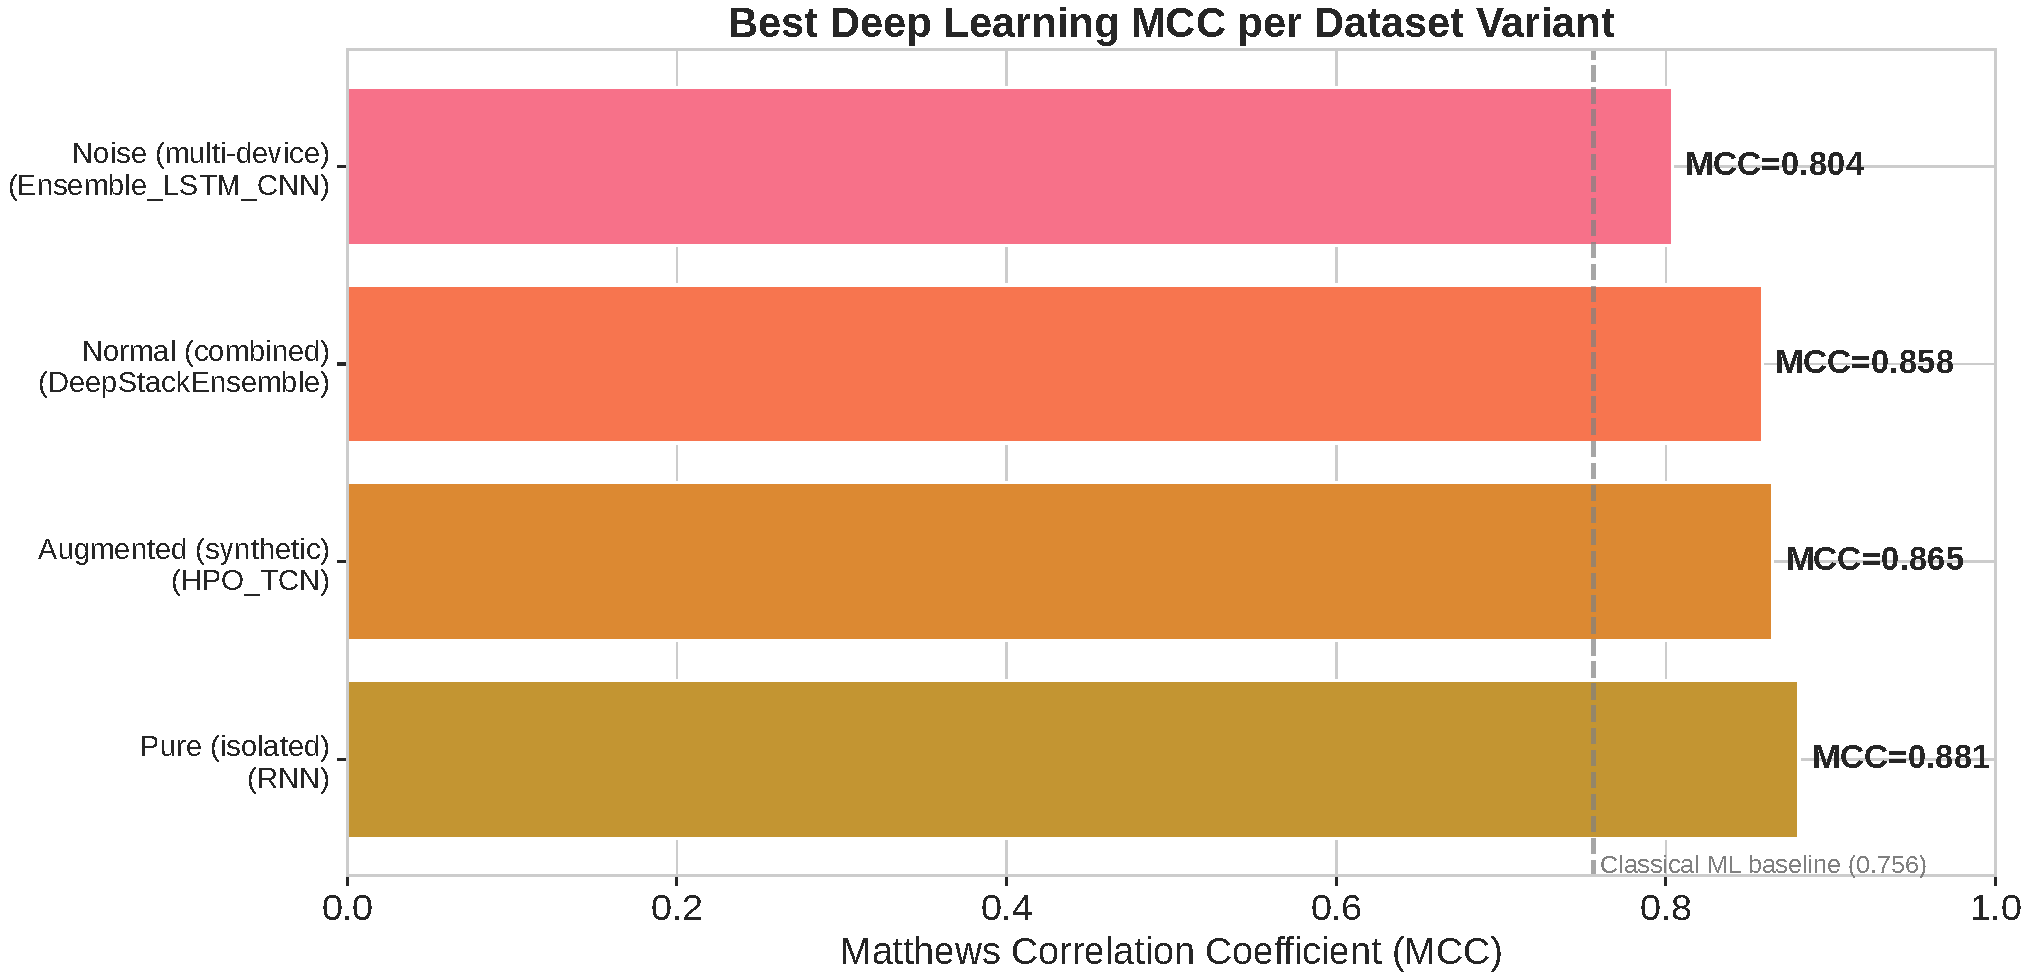
\includegraphics[width=0.80\columnwidth]{images/variant_mcc_comparison.pdf}
\caption{Best model MCC per variant. Classical baseline (0.756) dashed.}
\label{fig:variant_mcc}
\end{figure}

\subsection{Architecture Performance and HPO}

CNN (MCC 0.838) and TCN (0.836) lead single architectures; recurrent defaults underperform (RNN 0.755, GRU 0.710). Mamba (0.800) beats Transformer (0.713) by 12.2\% with $O(L)$ complexity. HPO yields large recurrent gains: GRU 0.710$\to$0.852 ($+$20.0\%), LSTM 0.686$\to$0.844 ($+$23.1\%), BiLSTM 0.684$\to$0.820 ($+$19.9\%). CNN/TCN gain less. Each model underwent 100 Optuna TPE trials; SoftMoE used NSGA-II.

Table~\ref{tab:combined_results} lists top models. DeepStackEnsemble (18 base models $\to$ per-class Level2Net $\to$ residual MetaMLP) achieves best combined MCC 0.859. Voting pairs improve over individuals (CNN$+$TCN 0.859 augmented); adding weaker models degrades (All-9: 0.807).

\begin{table}[H]
\centering
\caption{Top Models by Variant}
\label{tab:combined_results}
\resizebox{\columnwidth}{!}{\begin{tabular}{@{}lccc@{}}\toprule
\textbf{Model} & \textbf{Variant} & \textbf{MCC} & \textbf{Acc.} \\\midrule
DeepStackEnsemble  & Normal    & 0.8585 & 0.8937 \\
HPO GRU            & Normal    & 0.8524 & 0.8893 \\
HPO TCN            & Normal    & 0.8470 & 0.8843 \\
CNN                & Normal    & 0.8383 & 0.8774 \\\midrule
HPO TCN            & Augmented & 0.8647 & 0.8982 \\
HPO CNN            & Augmented & 0.8642 & 0.8977 \\
Ensemble CNN$+$TCN & Augmented & 0.8587 & 0.8932 \\\midrule
RNN                & Pure\textsuperscript{*}   & 0.8808 & 0.9063 \\\midrule
DS RNN\_B          & Noise\textsuperscript{*}  & 0.7981 & 0.8458 \\
HPO LSTM           & Noise\textsuperscript{*}  & 0.7908 & 0.8417 \\\bottomrule
\multicolumn{4}{c}{\footnotesize\textsuperscript{*}Seed~3.}\end{tabular}}
\end{table}

\subsection{Per-Class Performance}

Per-class F1 reveals consistent difficulty patterns. AB (alighting) leads (F1 0.893--0.925) due to distinctive descending trajectory; AA (inside) is hardest (0.831--0.894) from signal saturation near the AP; BB (at stop, 0.818--0.907) benefits from low RSSI; BA (boarding, 0.838--0.914) has moderate difficulty. Noise degrades AB most because concurrent near-AP transmissions mask its 20~dBm descent.

Figure~\ref{fig:cm} shows confusion matrices for the two best single-classification approaches. DeepStackEnsemble classifies 89.3\% correctly, with AA$\leftrightarrow$BA (both near-AP states) and AB$\leftrightarrow$BB (both exterior locations) as primary confusion pairs. CNN shows a qualitatively similar pattern with more off-diagonal errors, particularly misclassifying AA as AB near the AP.

\begin{figure}[H]
\centering
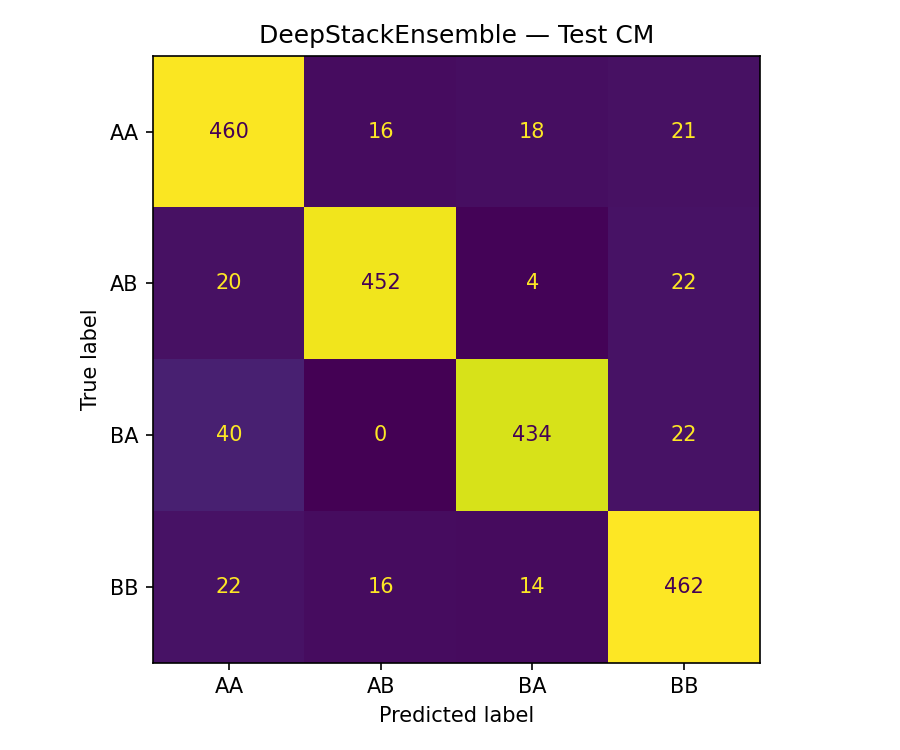
\includegraphics[width=0.42\textwidth]{images/cm_deepstack.png}\hfill
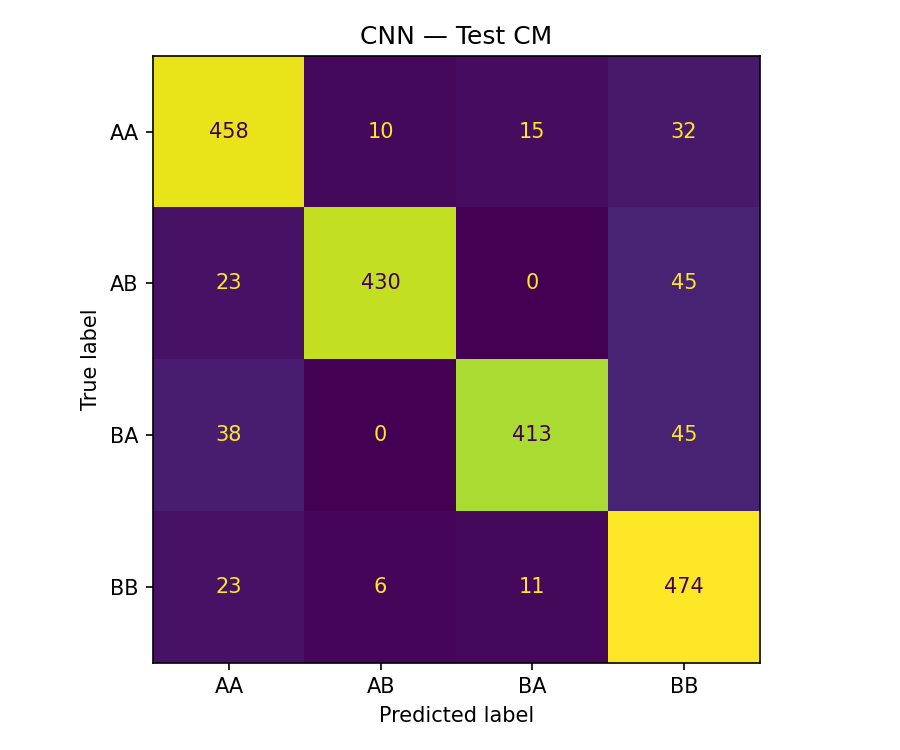
\includegraphics[width=0.42\textwidth]{images/cm_cnn.png}
\caption{Confusion matrices: DeepStackEnsemble (left, MCC 0.859) and CNN (right, MCC 0.838).}
\label{fig:cm}
\end{figure}

\subsection{Noise and Interference Analysis}

Figure~\ref{fig:interference_heatmap} quantifies mean RSSI shift per (Route $\times$ Interferer) pair. Three patterns emerge: (1) AA dominates as interferer ($+$45--53~dBm) because devices near the AP transmit at high power; BB causes minimal shift ($\le +$3.1~dBm). (2) AB is most affected ($+$46.6~dBm from AA): near-AP transmissions mask its descent. (3) Self-interference is minimal ($+$1.2--4.6~dBm).

\begin{figure}[H]
\centering
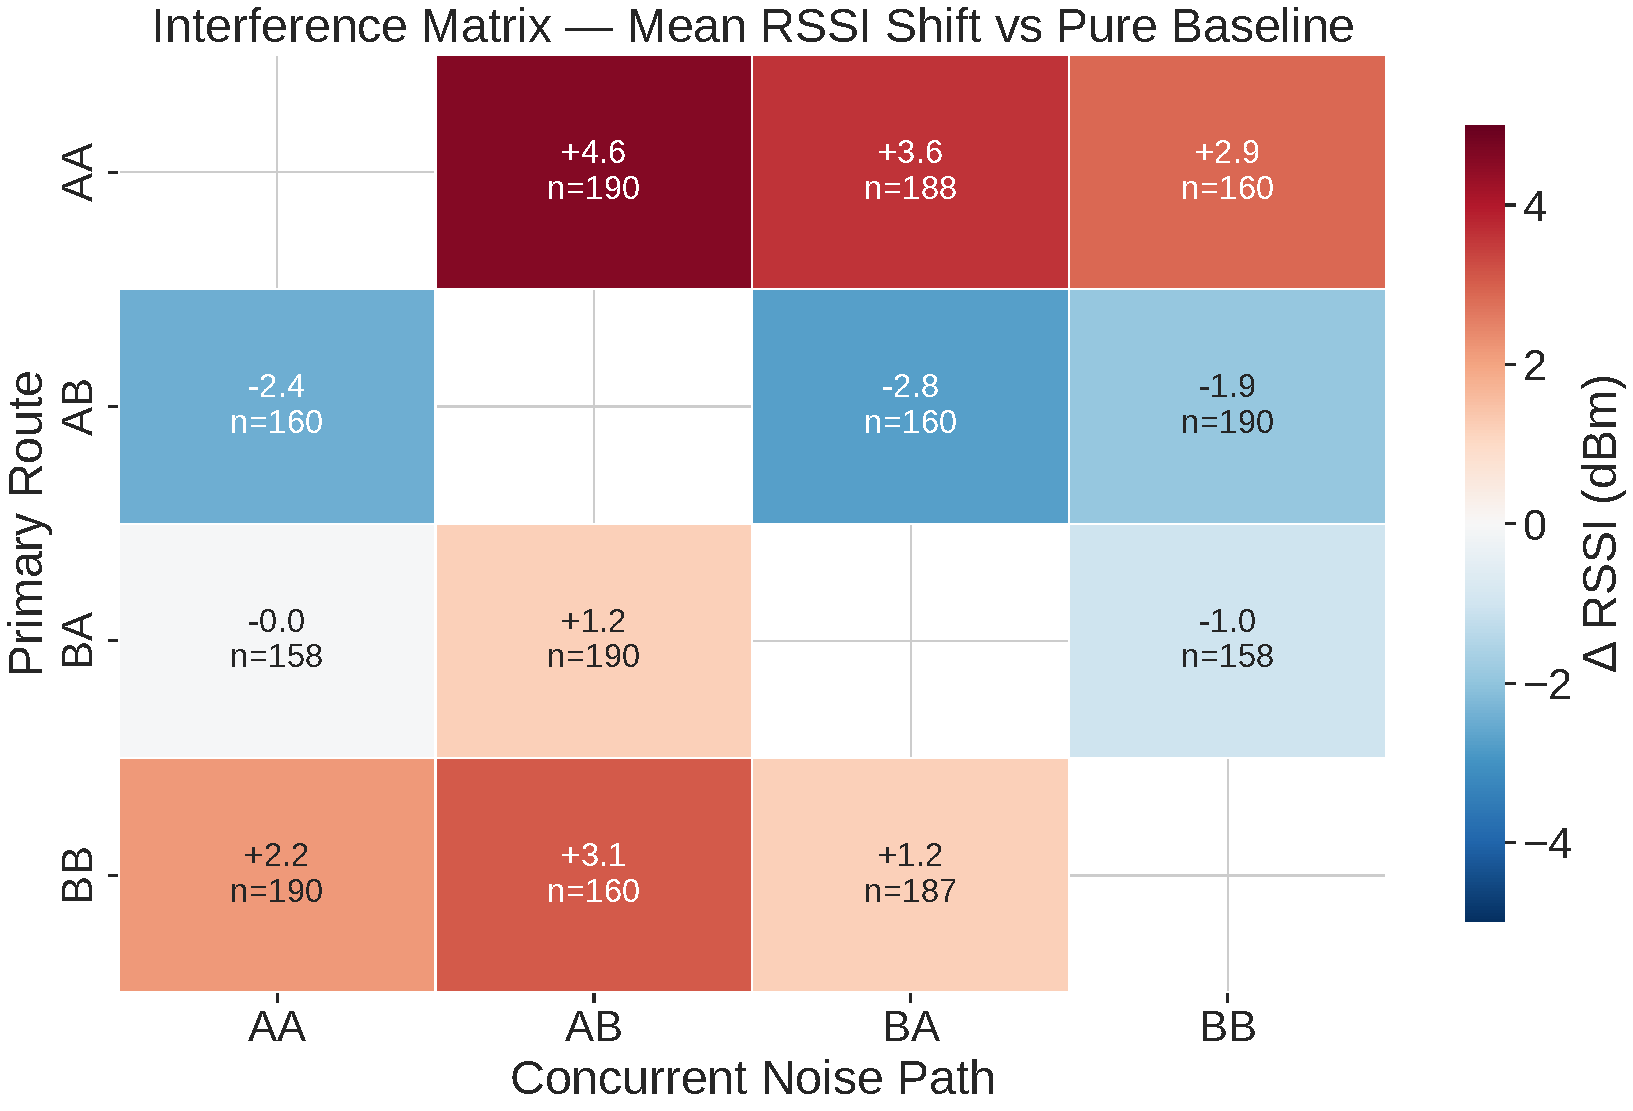
\includegraphics[width=0.85\columnwidth]{images/interference_heatmap.pdf}
\caption{Interference heatmap: AA dominates; self-interference minimal.}
\label{fig:interference_heatmap}
\end{figure}

Figure~\ref{fig:trajectories} explains \emph{why} each class degrades differently under interference. AA suffers from BA raising its stable high-RSSI profile, making near-AP states hard to separate. AB's 20~dBm descent is flattened by AA into a constant profile indistinguishable from AA---directly explaining AB's noise-induced F1 drop. BA's ascending trajectory is compressed by AA interference, reducing the distinctive 15~dBm ascent. BB's flat $-$50~dBm pattern shifts upward under AA but retains its shape, explaining BB's noise resilience: classification depends on temporal flatness, not absolute level.

\begin{figure}[H]
\centering
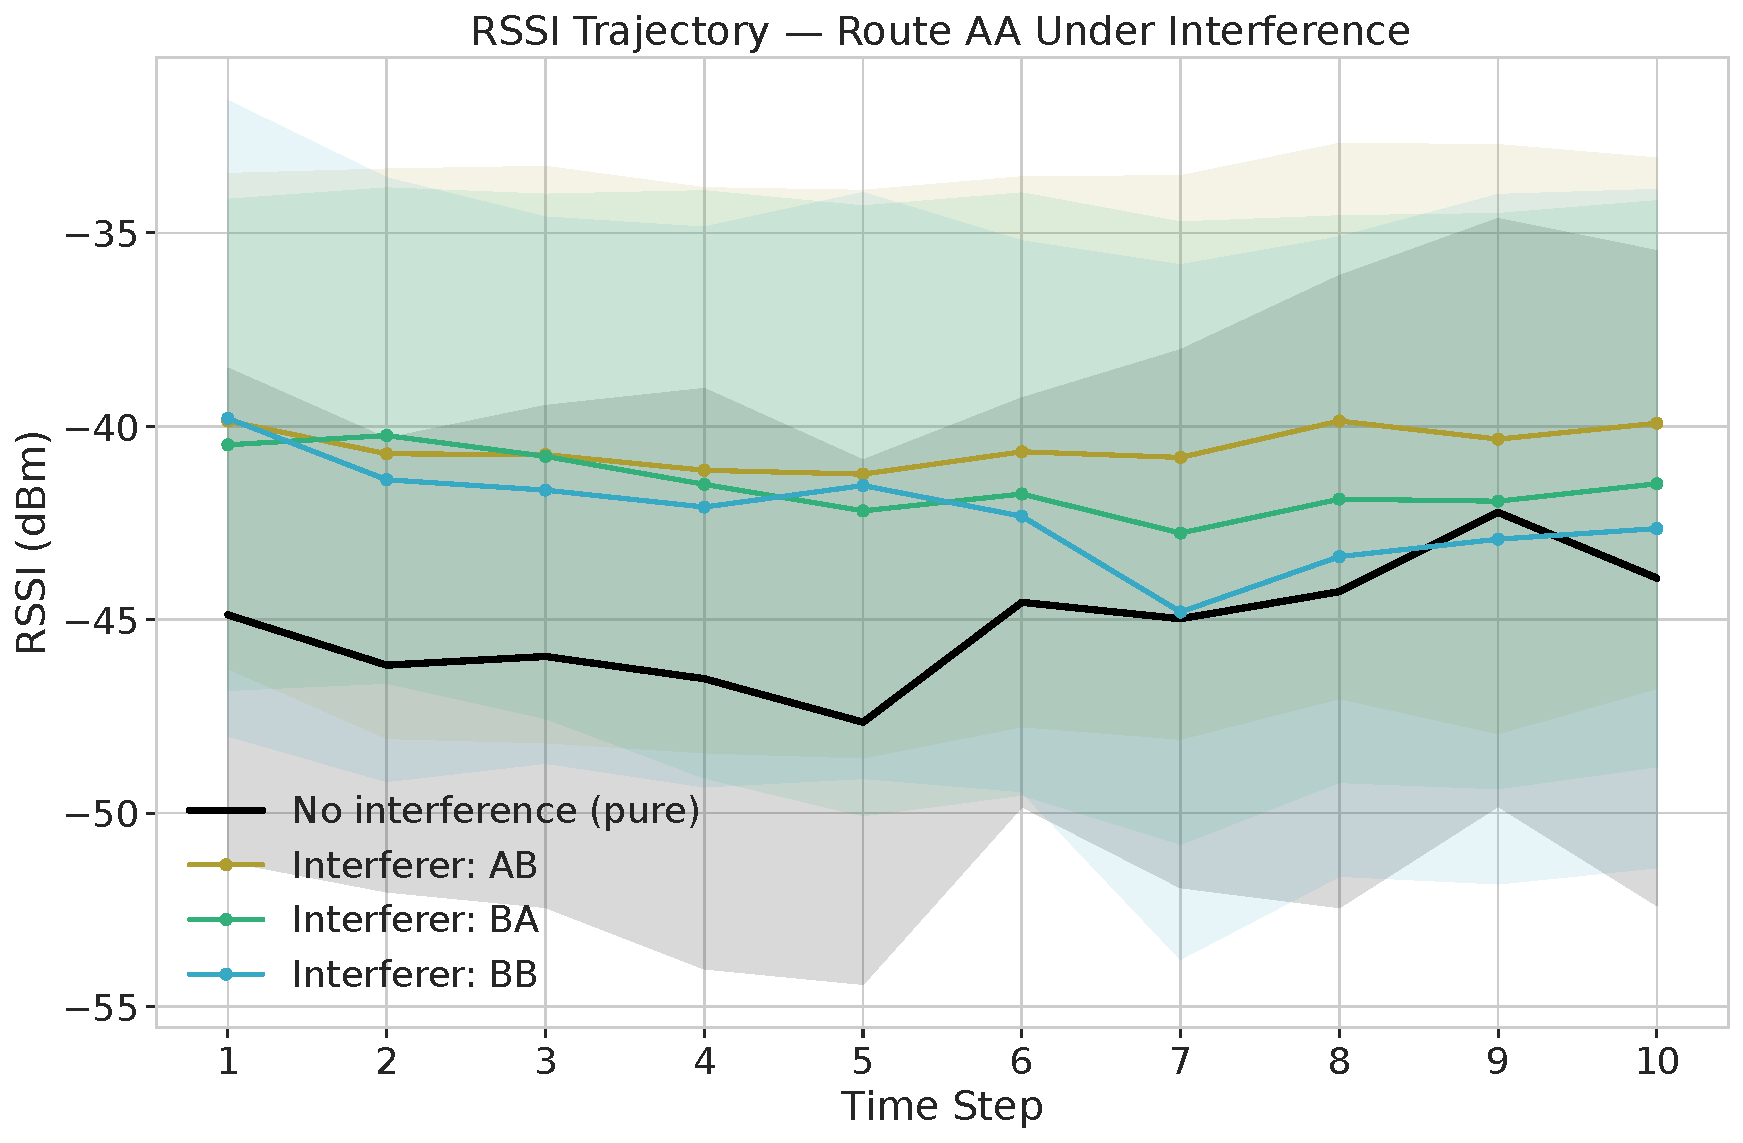
\includegraphics[width=0.45\textwidth]{images/interference_trajectory_AA.pdf}\hfill
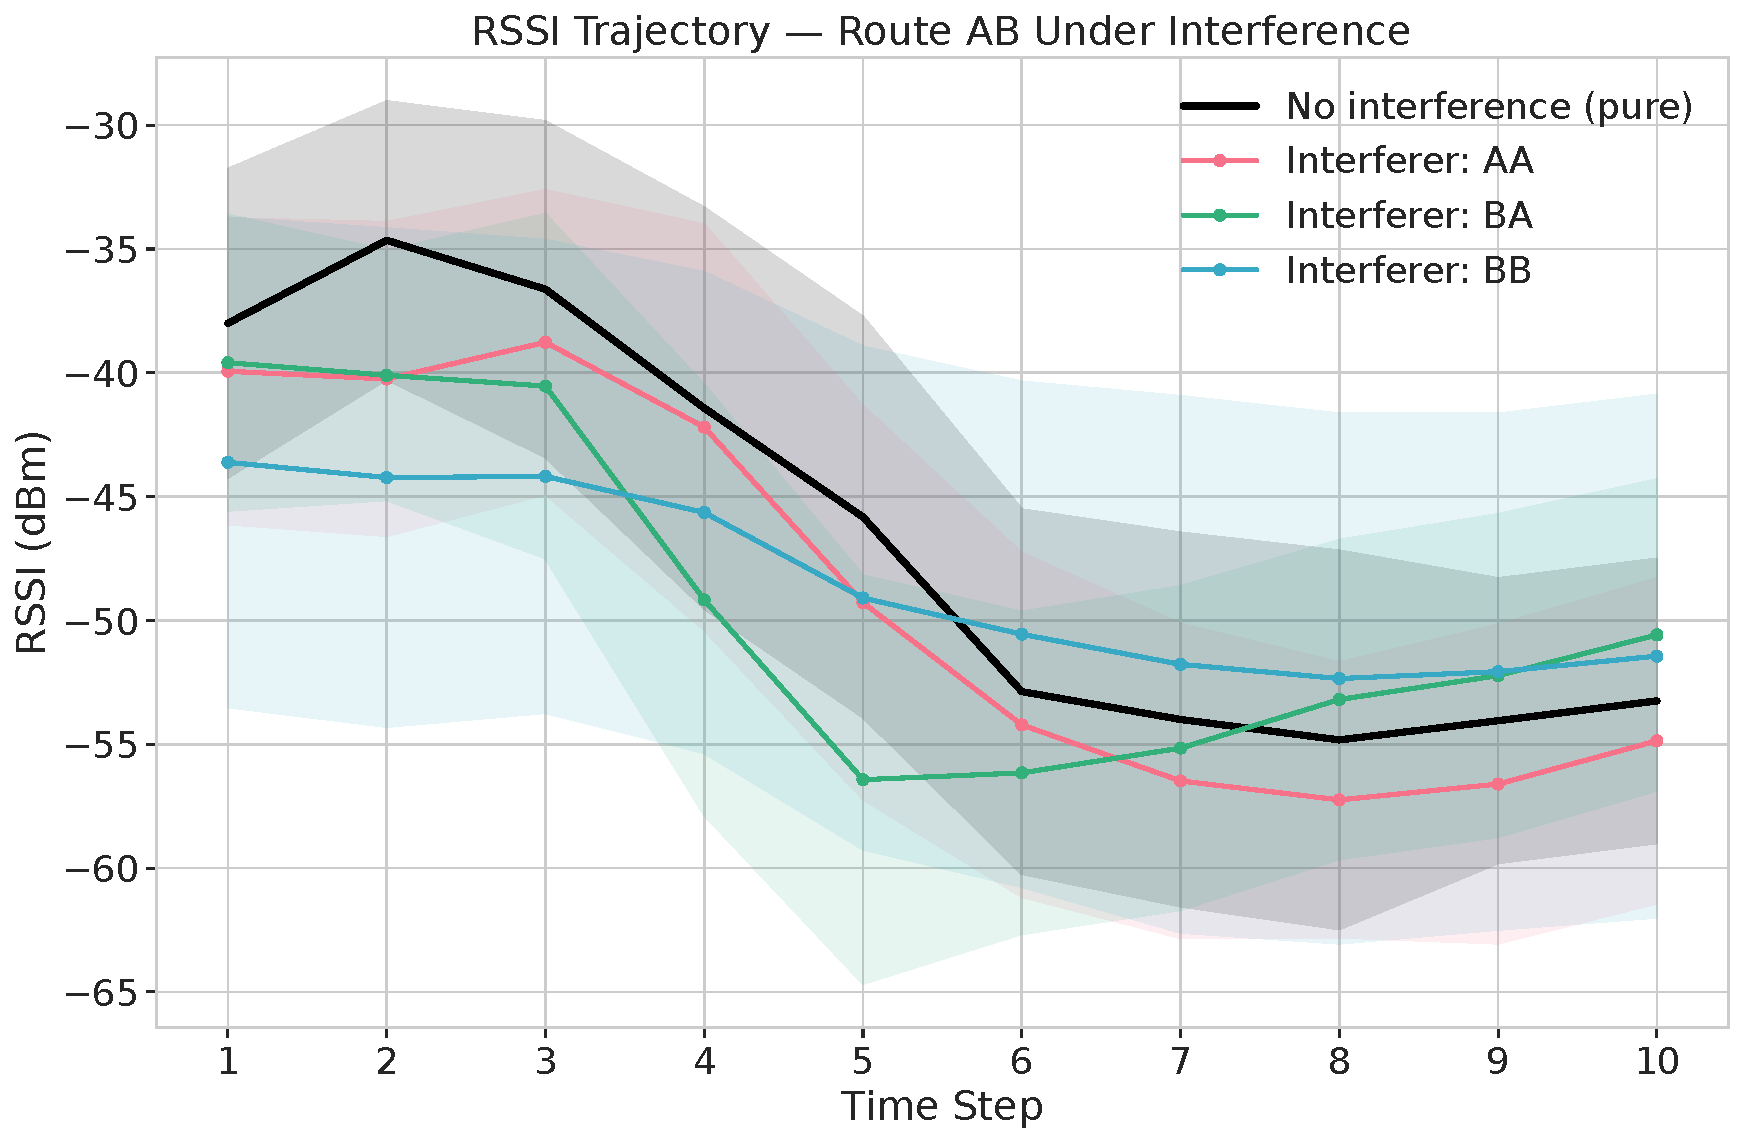
\includegraphics[width=0.45\textwidth]{images/interference_trajectory_AB.pdf}\\[4pt]
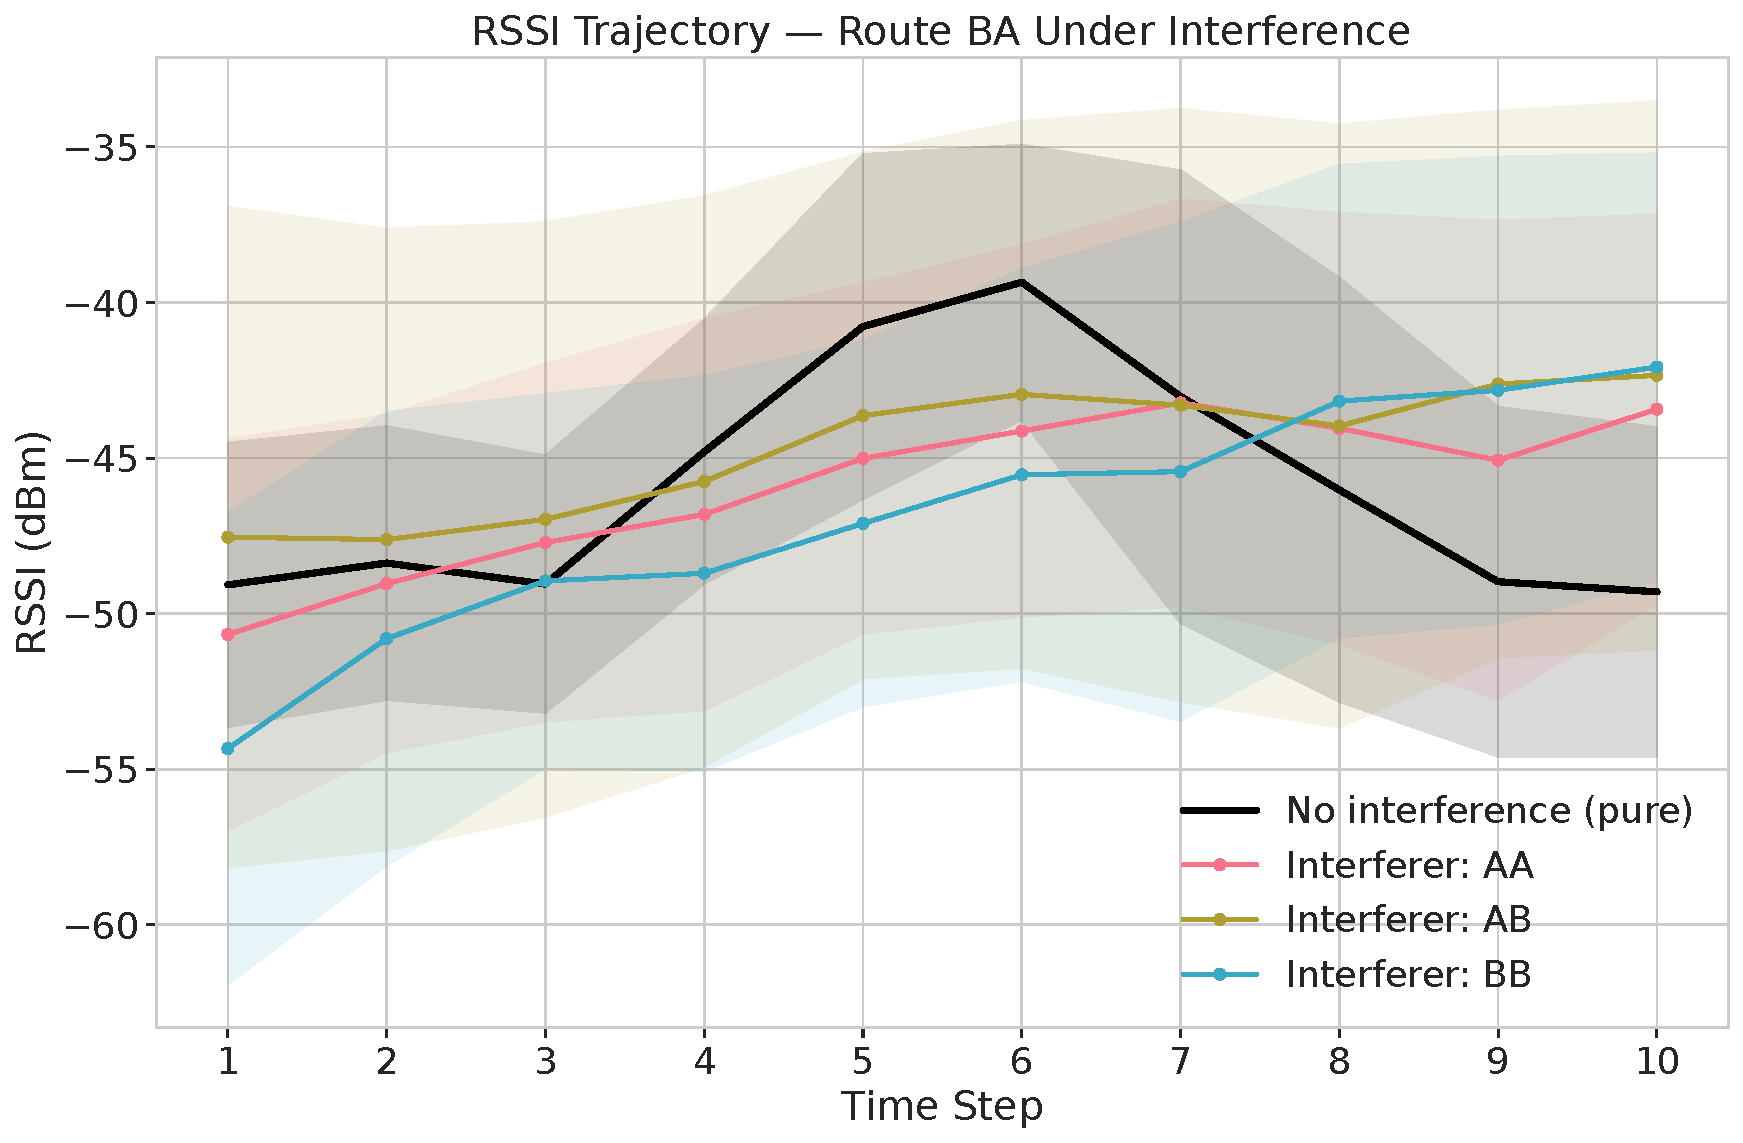
\includegraphics[width=0.45\textwidth]{images/interference_trajectory_BA.pdf}\hfill
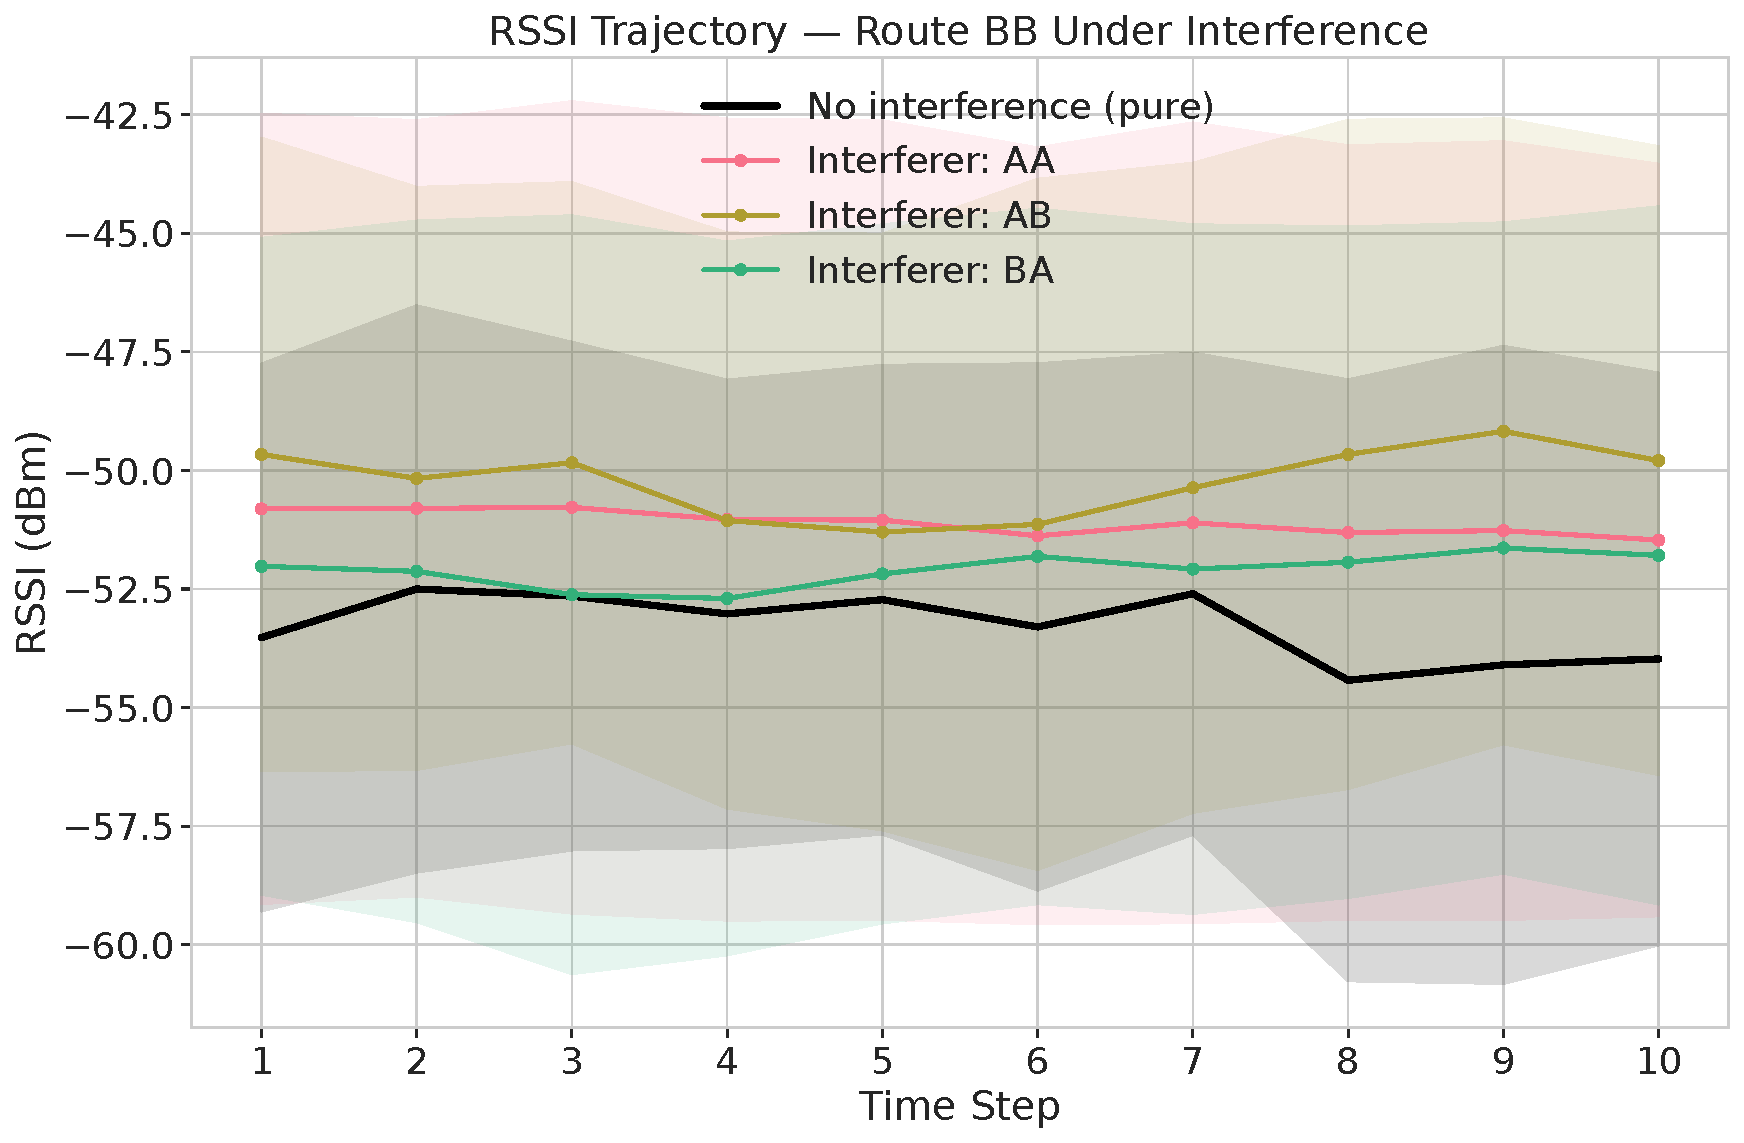
\includegraphics[width=0.45\textwidth]{images/interference_trajectory_BB.pdf}
\caption{Trajectories under interference. Top-left: AA---BA raises profile. Top-right: AB---AA masks descent entirely. Bottom-left: BA---AA compresses ascent. Bottom-right: BB---flat pattern persists despite shift.}
\label{fig:trajectories}
\end{figure}

Per-timestep analysis reveals perturbation peaks at timesteps~4--6 (closest to AP). MetaFusion\_GRU reaches MCC 0.783 on noise (vs.~0.758 for standard GRU) by encoding noise context, though the gap to pure (0.881) confirms that metadata alone cannot fully compensate for signal ambiguity under concurrent transmissions.

CNN (28K params, 129~s) offers the best efficiency-accuracy tradeoff among single models. Mamba (89K, 374~s) provides $O(L)$-complexity competitive accuracy. HPO GRU (198K, 107~s) is the strongest single model. DeepStackEnsemble (1.2M) suits server-side deployment.

\subsection{Feature Importance}

Permutation importance analysis across the 4 engineered channels and 10 timesteps, averaged over CNN, TCN, and GRU, reveals that window deviation---how far each timestep deviates from the per-sample mean---is the most informative channel (mean $\Delta$MCC $9.1\times 10^{-3}$), particularly at early timesteps ($t\!=\!1$--3) where it captures each class's characteristic offset from its baseline. This confirms that trajectory shape, not absolute magnitude, carries the strongest discriminative signal.

Velocity ($\Delta$) peaks at $t\!=\!4$ ($18.4\times 10^{-3}$), the mid-trajectory moment of maximum movement. Raw RSSI matters most at $t\!=\!6$, where absolute levels separate near-AP from exterior positions. Acceleration ($\Delta^2$) contributes at $t\!=\!3$--5, capturing directional movement onset. These results validate the 4-channel engineering strategy and align with the trajectory analysis in Figure~\ref{fig:trajectories}, where AB's defining 20~dBm descent occurs during timesteps~4--7.

\begin{figure}[H]
\centering
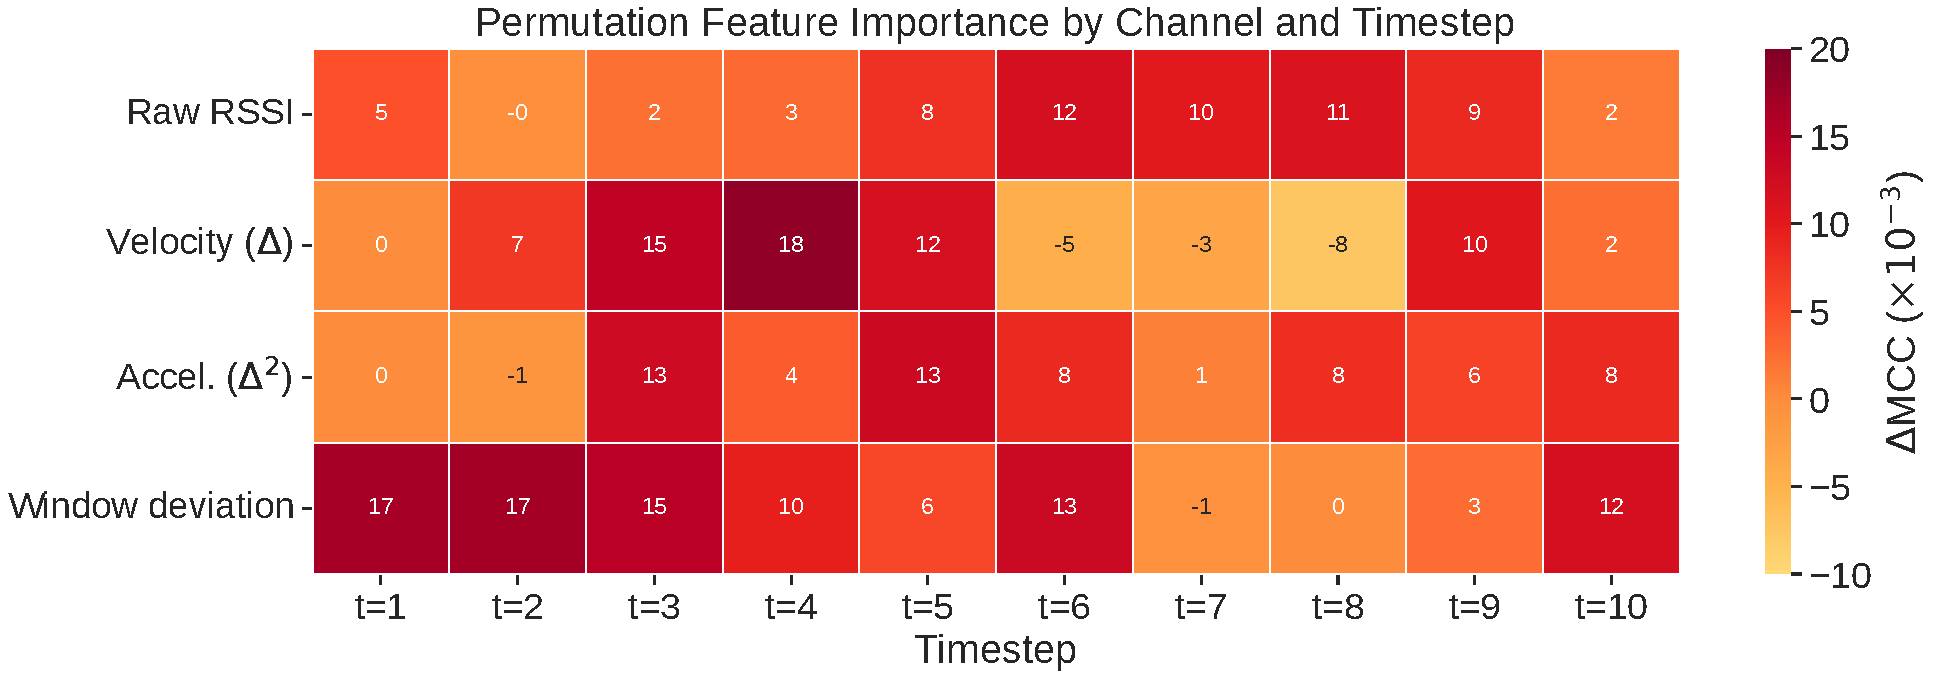
\includegraphics[width=0.85\columnwidth]{images/feature_importance_dl.pdf}
\caption{Permutation feature importance ($\Delta$MCC) across 4 channels $\times$ 10 timesteps, averaged over CNN, TCN, and GRU.}
\label{fig:feature_importance}
\end{figure}

\section{Conclusion}

This paper evaluated deep learning architectures for RSSI-based passenger movement classification in public transport. Building on classical ML baselines at MCC 0.756, we tested 11+ architectures spanning recurrent, convolutional, transformer, state-space, and mixture-of-experts models. The evaluation used four dataset variants, class-conditioned data augmentation, and exhaustive hyperparameter optimization.

The two-stage DeepStackEnsemble achieved MCC 0.859 and accuracy 89.4\% on combined data, a 13.6\% relative improvement. State-space models reached up to MCC 0.850 with $O(L)$ complexity, confirming their viability as an alternative to transformers for resource-constrained deployment.

Cross-route interference analysis revealed a 9.4\% absolute MCC degradation under multi-device noise. Heatmap analysis identified AA as the dominant interferer and AB as the most vulnerable route. Trajectory visualization showed that concurrent near-AP transmissions erase AB's characteristic 20~dBm RSSI descent. BB proved most noise-resilient because its classification signal comes from temporal flatness, which survives interference-level shifts intact.

Feature importance analysis confirmed and extended prior findings. Classical ML identified early timesteps as most informative. DL additionally captured mid-trajectory motion dynamics through the velocity channel, contributing directly to the 13.6\% improvement. Window deviation emerged as the most informative channel, explaining BB's noise resilience through shape-based classification.

Future work should explore attention mechanisms that learn to down-weight interfered timesteps. Multi-AP fusion could disambiguate near-AP states through spatial diversity. Integration of movement classification with origin-destination matrix inference would enable end-to-end passenger flow modeling. Context-aware architectures that jointly model signal and environmental metadata offer a promising direction for real-world deployment.


\section{Generative AI Declaration}
During the preparation of this manuscript, the authors used DeepSeek as a writing assistant for language improvement, grammar correction, and formatting. All technical content, experimental design, model architectures, results, analysis, and conclusions represent the authors' original intellectual contribution. The authors take full responsibility for the accuracy and integrity of the content. No AI-generated figures, fabricated citations, or manipulated results are present in this work.

\section*{Acknowledgment}
This work is supported by the European Regional Development Fund (FEDER), through the Regional Operational Programme of Centre (CENTRO 2030) of the Portugal 2030 framework [Project inMotion with Nr. 21359 (CENTRO2030-FEDER-02225900)].

\bibliographystyle{IEEEtran}
\bibliography{references}

\end{document}
